% Relatório de disciplina formatado com a classe-ifg (modo "relatorio").
% Compilação: pdflatex relatorio && bibtex relatorio && pdflatex relatorio && pdflatex relatorio
% (ou simplesmente: latexmk -pdf relatorio)
\documentclass[relatorio]{formatacao/classe-ifg}

% A classe fixa 12pt; o pacote scrextend permite trocar o tamanho-base da fonte
% (limite de páginas do relatório). Remova as duas linhas para voltar a 12pt.
\usepackage{scrextend}
\changefontsizes[13pt]{11pt}

% Estilo dos trechos de código (as cores pblue, pgreen e maroon vêm da classe)
\lstset{
  basicstyle=\scriptsize\ttfamily,
  keywordstyle=\color{pblue}\bfseries,
  commentstyle=\color{pgreen}\itshape,
  stringstyle=\color{maroon},
}

% "Fonte" para o ambiente codigo (a classe só define \fontefig, \fontetab e \fontequa)
\newcommand{\fontecod}[1]{\par\vspace{-0.15cm}{\footnotesize\centering Fonte: #1.\par}}

% Flutuantes (figuras, tabelas, quadros e códigos) são despejados antes das
% referências (\FloatBarrier no fim do documento), para que nenhum fique depois
% delas. Os parâmetros abaixo deixam o LaTeX encher melhor as páginas com texto
% e flutuantes, em vez de deixar meias páginas em branco.
\usepackage{placeins}
\renewcommand{\topfraction}{0.9}
\renewcommand{\bottomfraction}{0.8}
\renewcommand{\textfraction}{0.07}
\renewcommand{\floatpagefraction}{0.7}
\setcounter{topnumber}{4}
\setcounter{bottomnumber}{3}
\setcounter{totalnumber}{6}

% Colunas de texto alinhadas à esquerda (tabularx e tabular)
\newcolumntype{Y}{>{\raggedright\arraybackslash}X}
\newcolumntype{P}[1]{>{\raggedright\arraybackslash}p{#1}}

\hypersetup{
  pdftitle={Triagem da gravidade de acidentes em rodovias federais com Multilayer Perceptrons},
  pdfauthor={Igor Coutinho Ferreira Nobre},
  pdfsubject={Relatório técnico - Deep Learning}
}

\hyphenation{hi-per-pa-râ-me-tros re-gu-la-ri-za-ção}

% Compactação (limite de páginas do relatório): linhas de tabela sem altura
% extra, menos espaço em volta de flutuantes e de trechos de código.
\setlength{\extrarowheight}{1.5pt}
\setlength{\floatsep}{6pt plus 2pt minus 2pt}
\setlength{\textfloatsep}{8pt plus 2pt minus 2pt}
\setlength{\intextsep}{6pt plus 2pt minus 2pt}
\setlength{\abovecaptionskip}{3pt}
\setlength{\belowcaptionskip}{2pt}
\lstset{aboveskip=4pt, belowskip=6pt}
% Títulos de capítulo com menos espaço vertical (a classe usa 20pt antes e 40pt depois)
\makeatletter
\def\@makechapterhead#1{%
  \vspace*{6\p@}%
  {\interlinepenalty\@M
   \par\nobreak
   \raggedright\Large\rm\bfseries\MakeUppercase{\thechapter\space\space\space\space\space#1}\par\nobreak
   \vskip 10\p@
  }}
\def\@makeschapterhead#1{%
  \vspace*{6\p@}%
  {\interlinepenalty\@M
   \par\nobreak
   \raggedright\Large\rm\bfseries\MakeUppercase{#1}\par\nobreak
   \vskip 10\p@
  }}
% Seções e subseções com menos espaço vertical (padrão do report: 3,5ex antes e 2,3ex depois)
\renewcommand\section{\@startsection{section}{1}{\z@}%
  {-2.2ex \@plus -1ex \@minus -.2ex}{1.2ex \@plus .2ex}{\normalfont\Large\bfseries}}
\renewcommand\subsection{\@startsection{subsection}{2}{\z@}%
  {-1.8ex \@plus -1ex \@minus -.2ex}{0.8ex \@plus .2ex}{\normalfont\large\bfseries}}
\makeatother

% Sem os números de página de retrocitação ao fim de cada referência
\renewcommand*{\backref}[1]{}
\renewcommand*{\backrefalt}[4]{}
% Referências em fonte um pouco menor e com menos espaço entre itens
\AtBeginEnvironment{thebibliography}{\footnotesize\setlength{\itemsep}{2pt}}

%INICIO DO DOCUMENTO ---------------------------------------------- %
\begin{document}

% -------- Autor
\autor{Igor Coutinho Ferreira Nobre}
% -------- Título e subtítulo
\titulo{Triagem da gravidade de acidentes em rodovias federais com Multilayer Perceptrons}
\subtitulo{Classificação multiclasse sobre os dados abertos da PRF (2007 a 2026), com busca de hiperparâmetros via Optuna}
% -------- Curso (a folha de rosto imprime "\tipocurso em \curso")
\tipocurso{Especialização}
\curso{Inteligência Artificial Aplicada}
% -------- Disciplina (usado apenas no relatório de disciplina)
\disciplina{Deep Learning -- Frente 3.1: Multilayer Perceptrons}
% -------- Local e data
\campus{Goiânia}
\dia{15}
\mes{10}
\ano{2026}
% -------- Professor da disciplina (no modo relatorio é impresso como "Professor:")
\orientador{Prof. Dr. Sérgio Canuto}
\unidade{IFG / Câmpus Goiânia}

% Elementos pré-textuais. No modo "relatorio" a classe não gera capa separada,
% ficha, termo, folha de aprovação nem listas de figuras/tabelas: a folha de
% rosto é seguida do resumo e o texto corre sem quebra de página entre capítulos.
\rosto
\tabelas % no modo relatorio imprime apenas o Resumo (arquivo pre/preResumo.tex)
\singlespacing % corpo do texto em espaçamento simples (limite de páginas do relatório)

% Corpo do texto
\chapter{Introdução e objetivo}
\label{cap:intro}

Quando alguém liga para a Polícia Rodoviária Federal (PRF) para relatar um acidente, a central precisa decidir, com pouca informação, o que enviar: só uma viatura e um guincho, ou também ambulância e resgate. Este trabalho treina uma \textit{Multilayer Perceptron} (MLP) para estimar a gravidade do acidente a partir do que se sabe da ocorrência antes da contagem de vítimas: tipo de acidente, causa provável, quantidade de veículos e pessoas envolvidos, local, horário e condições da via (a causa é avaliação da equipe, não do solicitante; Seção~\ref{sec:selecao}). A previsão serve para ordenar as ocorrências por risco e priorizar o despacho; o modelo apoia a decisão, não a substitui.

A unidade de observação é um acidente (uma linha dos arquivos anuais da PRF). A variável alvo é \texttt{classificacao\_acidente}, com três classes mutuamente exclusivas: \texttt{Sem Vítimas}, \texttt{Com Vítimas Feridas} e \texttt{Com Vítimas Fatais}. Trata-se, portanto, de um problema de classificação multiclasse. Entre as frentes propostas, foi escolhida a de \textit{Multilayer Perceptrons}.

O código foi escrito em Python 3.12, com PyTorch 2.14 para a rede, scikit-learn 1.9 para o pré-processamento e as métricas, e Optuna 5.0 para a busca de hiperparâmetros. Tudo foi executado em CPU (Apple M1 Pro, 16 GB), com sementes fixas. O notebook, os artefatos e o registro completo da busca estão no repositório \url{https://github.com/coutinhonobre/Trabalho-Final---Pos-Deep-Learning} \cite{nobre2026}.

\chapter{Descrição da fonte e caracterização do conjunto de dados}
\label{cap:dados}

\section{Fonte e variáveis}
\label{sec:entradas}

Foi utilizado o conjunto \textit{Acidentes nas Rodovias Federais (agrupados por ocorrência)}, publicado pela PRF no Portal Brasileiro de Dados Abertos \cite{prf2026}: um arquivo CSV por ano, de 2007 a 2026, com uma linha por acidente, somando 2.237.189 registros. As 12 entradas, todas categóricas, estão no Quadro~\ref{qua:entradas}, em três grupos. As contagens de pessoas e veículos têm caudas longas (mediana 2, mas até 248 pessoas e 131 veículos num registro) e foram convertidas em faixas, que é também o que um solicitante consegue informar.

\begin{quadro}[!htbp]
\caption{Variáveis de entrada}
\label{qua:entradas}
\begin{center}
\footnotesize
\begin{tabularx}{\textwidth}{|P{1.7cm}|l|P{1.45cm}|P{2.9cm}|Y|}
\hline
\textbf{Grupo} & \textbf{Variável} & \textbf{Categorias} & \textbf{Mais frequente} & \textbf{Observação} \\ \hline
\multirow{4}{1.7cm}{Contexto da via}
 & \texttt{condicao\_metereologica} & 10 & céu claro (52\%) & \texttt{ignorado} mantido como valor legítimo \\ \cline{2-5}
 & \texttt{tipo\_pista} & 3 & simples (52\%) & simples, dupla, múltipla \\ \cline{2-5}
 & \texttt{tracado\_via} & 4 & reta (70\%) & multirrótulo desde 2017, reduzido à geometria principal \\ \cline{2-5}
 & \texttt{fase\_dia} & 4 & pleno dia (57\%) & \\ \hline
\multirow{4}{1.7cm}{Quando e onde}
 & \texttt{uf} & 27 & MG (14\%) & \\ \cline{2-5}
 & \texttt{br} & 213 (105 após agrupar raras) & 101 e 116 (17\% cada) & número da rodovia tratado como rótulo \\ \cline{2-5}
 & \texttt{fim\_de\_semana} & 2 & não (53\%) & derivada de \texttt{dia\_semana} (sexta a domingo) \\ \cline{2-5}
 & \texttt{periodo\_dia} & 4 & tarde (32\%) & derivada de \texttt{horario} (faixas de 6 h) \\ \hline
\multirow{4}{1.7cm}{Relato do solicitante}
 & \texttt{tipo\_acidente} & 19 & colisão traseira (25\%) & sinônimos entre formatos unificados \\ \cline{2-5}
 & \texttt{macro\_causa} & 7 & desatenção\slash manobra (44\%) & agrupa as até 75 causas detalhadas \\ \cline{2-5}
 & \texttt{veiculos\_cat} & 4 & 2 (51\%) & faixas 1, 2, 3, 4+ \\ \cline{2-5}
 & \texttt{pessoas\_cat} & 5 & 2 (48\%) & faixas 1, 2, 3, 4, 5+ \\ \hline
\end{tabularx}
\end{center}
\fontequa{Elaborado pelo autor}
\end{quadro}

\section{Qualidade dos dados e distribuição do alvo}
\label{sec:alvo}

A base tem poucos problemas: no máximo 70 ausentes por coluna de entrada, 11.697 linhas (0,52\%) com alvo ausente ou \texttt{Ignorado} e 6 duplicatas exatas; o \texttt{id} se repete entre anos e foi ignorado. As contagens de vítimas são coerentes com o rótulo (todo \texttt{Com Vítimas Fatais} tem mortos $>$ 0), e os 1.081 acidentes com 10 ou mais veículos são engavetamentos plausíveis, absorvidos pela faixa \texttt{4+}. Foram removidas 11.875 linhas (0,53\%), restando 2.225.314 acidentes.

O alvo é desbalanceado (Figura~\ref{fig:alvo}): \texttt{Com Vítimas Feridas} 48,4\%, \texttt{Sem Vítimas} 46,7\% e \texttt{Com Vítimas Fatais} 4,9\%. A fração de \texttt{Sem Vítimas} cai de cerca de 60\% até 2014 para cerca de 16\% a partir de 2019: uma mudança no procedimento de registro, não no perfil dos acidentes.

\begin{figure}[!htbp]
  \centering
  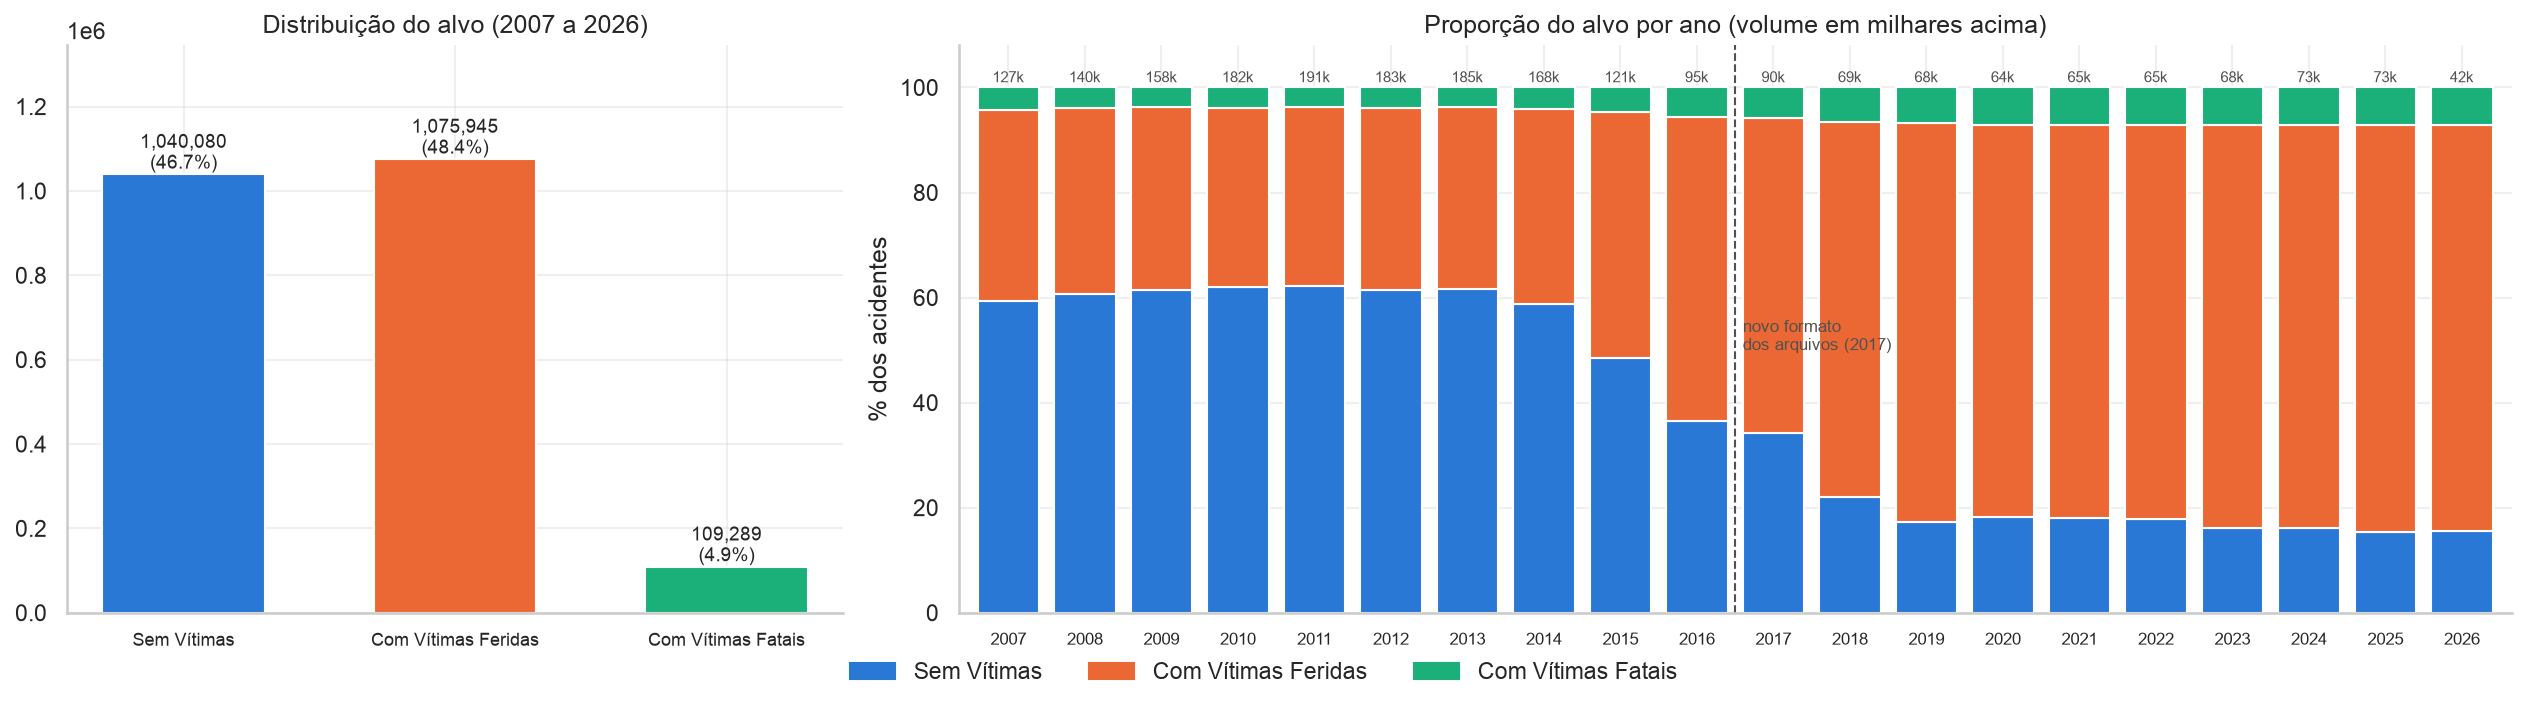
\includegraphics[width=0.7\textwidth]{figuras/01_alvo}
  \caption{Distribuição do alvo e proporção por ano}
  \label{fig:alvo}
  \fontefig{Elaborado pelo autor}
\end{figure}

A hora e o dia da semana importam (Figura~\ref{fig:hora-dia}): a taxa de fatais chega a 9\% na madrugada, contra cerca de 3\% entre 7 h e 17 h, e sobe no sábado (5,8\%) e no domingo (6,7\%), contra cerca de 4,3\% nos demais dias. Isso motivou derivar \texttt{periodo\_dia} e \texttt{fim\_de\_semana} (esta última agrupando sexta, sábado e domingo, os dias de maior volume). A mesma figura, à direita, compara, para cada entrada, a taxa de fatais da categoria mais letal com a da menos letal: as variáveis do relato do solicitante separam muito mais (27,9 p.p. em \texttt{tipo\_acidente}) que as de contexto da via (4 a 5 p.p.).

\begin{figure}[!htbp]
  \centering
  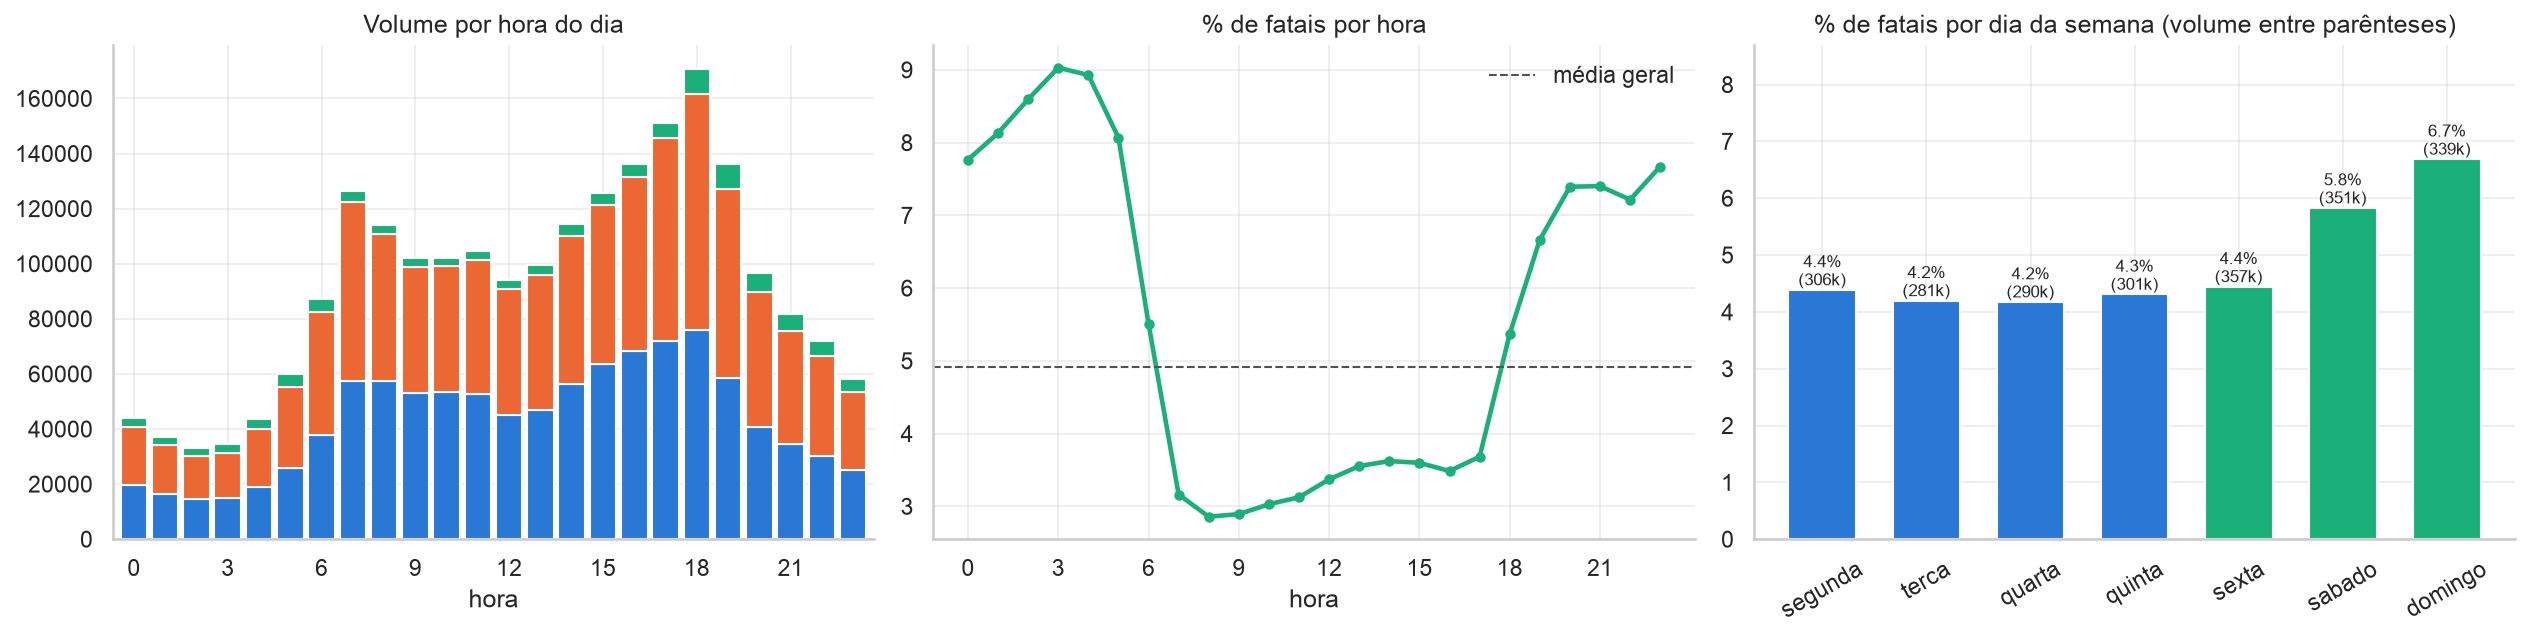
\includegraphics[width=0.6\textwidth]{figuras/02_hora_dia_semana}\hfill
  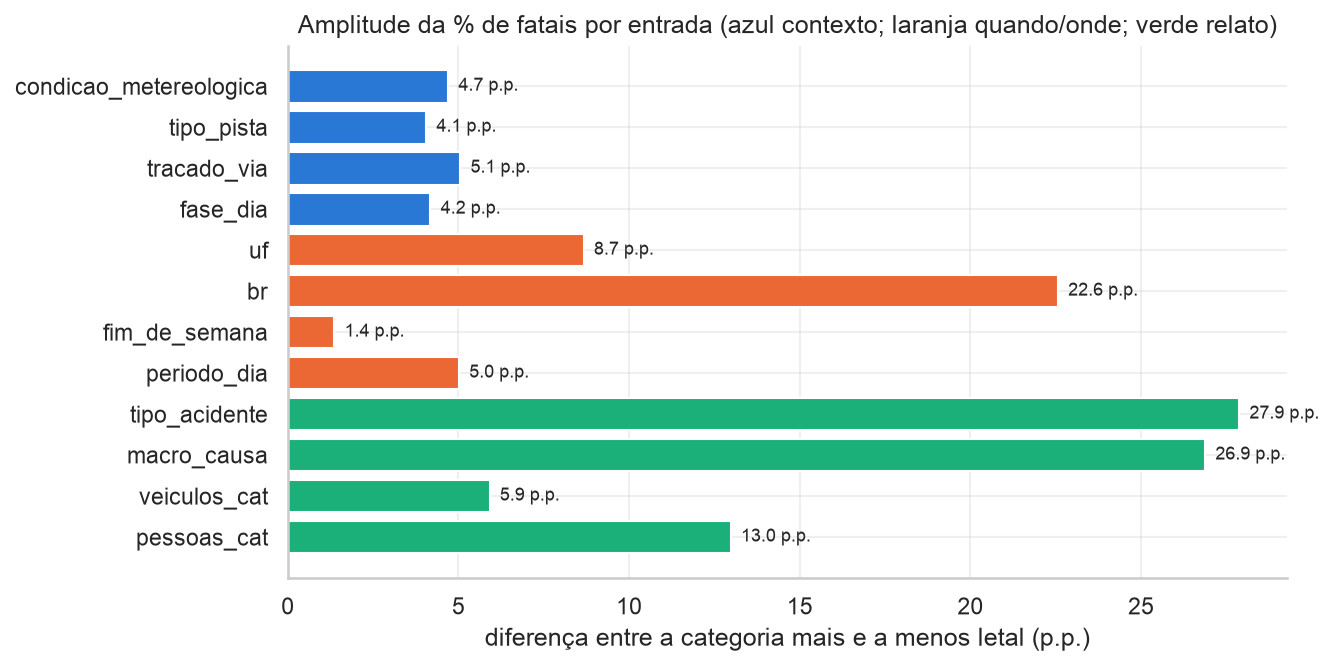
\includegraphics[width=0.38\textwidth]{figuras/09_amplitude_fatais}
  \caption{À esquerda, volume por hora e taxa de fatais por hora e por dia da semana; à direita, amplitude da taxa de fatais por entrada}
  \label{fig:hora-dia}
  \fontefig{Elaborado pelo autor}
\end{figure}

\section{Seleção de atributos e risco de vazamento}
\label{sec:selecao}

As contagens de vítimas (\texttt{mortos}, \texttt{feridos}, \texttt{ilesos} etc.) definem o rótulo e foram excluídas: seriam vazamento direto. Para que o modelo não aprendesse o período de registro em vez da gravidade, saíram também o \texttt{ano} e os campos que só existem a partir de 2017 (coordenadas, \texttt{regional}, \texttt{delegacia}, \texttt{uop}), e a causa detalhada, cujo vocabulário cresce de 11 valores em 2016 para 75 em 2023, foi agrupada em 7 macrocausas. \texttt{km}, \texttt{municipio} e \texttt{sentido\_via} saíram por cardinalidade alta ou pouca informação depois de \texttt{uf} e \texttt{br}. \texttt{causa\_acidente} é avaliação da equipe, não do solicitante, e pode não existir na triagem; seu efeito isolado não foi medido (Capítulo~\ref{cap:conclusao}).

\section{Divisão dos dados e pré-processamento}
\label{sec:preproc}

Os dados foram divididos em 70\% treino (1,56 milhão), 15\% validação (334 mil) e 15\% teste (334 mil), com estratificação pelo alvo. A divisão é aleatória porque não há unidades com várias observações, mas mistura no teste os dois regimes de registro da Seção~\ref{sec:alvo}: a estimativa vale para a distribuição histórica, não para o uso futuro. A validação cruzada não foi usada pelo custo com 2,2 milhões de linhas. O teste não participa de nenhuma seleção.

As entradas foram codificadas com \texttt{OneHotEncoder} ajustado somente no treino; categorias com menos de 200 ocorrências ou nunca vistas vão para uma coluna \aspas{infrequente}. O resultado são 194 colunas binárias, sem necessidade de normalização. Para o desbalanceamento, a perda recebe pesos de classe calculados no treino, com raiz quadrada aplicada (0,845 / 0,830 / 2,605): o peso integral ($\approx$6,8 para fatais) faria o modelo prever fatal em excesso. O expoente 0,5 foi fixado, não buscado, e define o ponto de operação entre \textit{recall} e precisão dos fatais.

\chapter{Arquiteturas, espaço de busca e protocolo de hiperparametrização}
\label{cap:metodologia}

\section{Arquitetura e treinamento}
\label{sec:arquitetura}

A MLP foi implementada em PyTorch como uma sequência configurável de blocos \texttt{Linear} $\rightarrow$ \texttt{ReLU} $\rightarrow$ \texttt{Dropout} (Código~\ref{cod:mlp}): 194 neurônios de entrada (as colunas \textit{one-hot}), camadas ocultas definidas pela busca e 3 neurônios de saída, um por classe, com softmax embutida na \texttt{CrossEntropyLoss} ponderada, a configuração usual para classificação multiclasse \cite{geron2019}. A ReLU não satura para valores positivos e é barata \cite{goodfellow2016}; o otimizador é o Adam; a inicialização é a padrão do PyTorch (variante da inicialização de He), que já preserva a variância das ativações com ReLU \cite{geron2019}. A Figura~\ref{fig:arq-m1} mostra o modelo final.

\begin{codigo}[!htbp]
  \lstinputlisting[language=Python]{prog/cod02-mlp.py}
  \fontecod{Elaborado pelo autor}
  \caption{Definição da MLP}
  \label{cod:mlp}
\end{codigo}

\begin{figure}[!htbp]
  \centering
  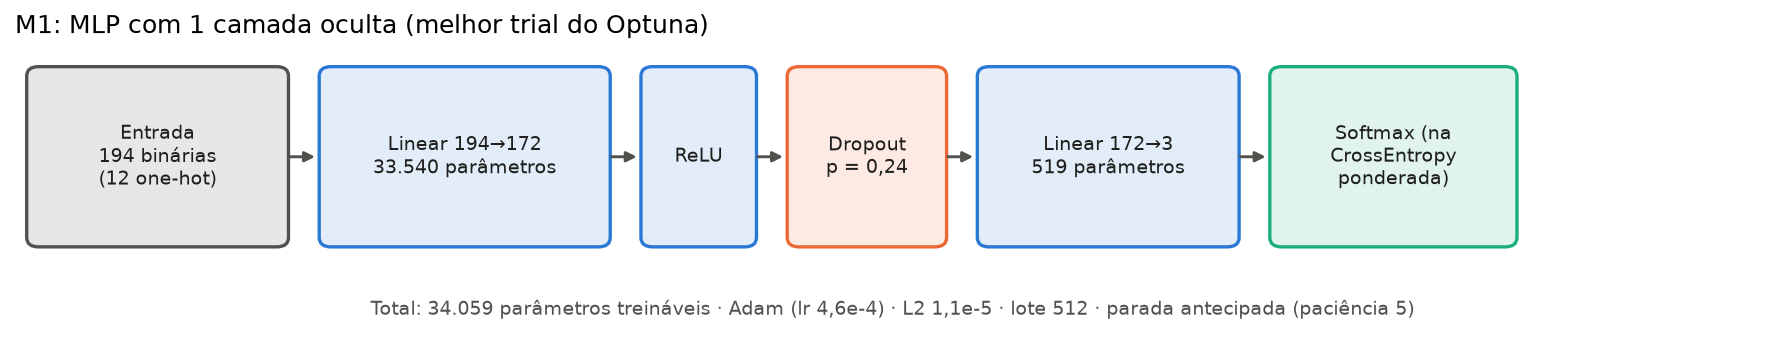
\includegraphics[width=0.62\textwidth]{figuras/16_arquitetura_m1}
  \caption{Arquitetura do modelo final (M1)}
  \label{fig:arq-m1}
  \fontefig{Elaborado pelo autor}
\end{figure}

Uma única função de treino, por épocas e \textit{mini-batches} com retropropagação do gradiente \cite{nielsen2015}, é usada na busca e nos modelos finais, com quatro regularizações: dropout após cada ReLU, L2 (\texttt{weight\_decay}), L1 (somada à perda como $\lambda \sum |w|$) e parada antecipada pelo Macro F1 de validação, que restaura os pesos da melhor época (paciência 4 na busca, 5 no treino final). A normalização por lote (BatchNorm) foi avaliada (Seção~\ref{sec:regularizacao}), mas não entrou nos modelos finais.

\section{Hiperparametrização: espaço de busca e configuração do estudo}
\label{sec:optuna}

A estratégia foi a busca bayesiana (\textit{Bayesian Search}), com o Optuna. Ao contrário do \textit{grid search}, que percorre toda a grade, e do \textit{random search}, que sorteia às cegas, ela usa os resultados anteriores para escolher a próxima tentativa: o amostrador TPE (\textit{Tree-structured Parzen Estimator}) concentra as tentativas nas regiões do espaço que vêm dando bons resultados. Isso importa aqui porque cada tentativa treina uma rede e o espaço tem sete hiperparâmetros.

Foram 25 tentativas, orçamento definido pelo tempo em CPU e suficiente porque as melhores convergem para a mesma região (Seção~\ref{sec:busca}), cada uma treinada numa subamostra estratificada de 300 mil linhas por até 15 épocas e avaliada na validação completa; o \texttt{MedianPruner} interrompe, a partir da 5\textsuperscript{a} época, as tentativas abaixo da mediana. A métrica otimizada foi o Macro F1 de validação, que dá o mesmo peso às três classes. O Quadro~\ref{qua:espaco} apresenta o espaço de busca e a justificativa de cada intervalo; otimizador, ativação e inicialização ficaram fora da busca por baixa influência esperada numa MLP rasa com entradas binárias.

\begin{quadro}[!htbp]
\caption{Espaço de busca e justificativa dos intervalos}
\label{qua:espaco}
\begin{center}
\footnotesize
\begin{tabularx}{\textwidth}{|P{2.6cm}|P{3.2cm}|Y|}
\hline
\textbf{Hiperparâmetro} & \textbf{Intervalo} & \textbf{Justificativa} \\ \hline
Taxa de aprendizado & $10^{-4}$ a $5 \cdot 10^{-3}$, escala log & em torno do padrão do Adam ($10^{-3}$), uma década abaixo e meia acima \\ \hline
Camadas ocultas & 1 a 3 & o teorema da aproximação universal \cite{hornik1989} garante uma camada em princípio, sem dizer quantos neurônios; mais camadas podem representar a mesma função com menos neurônios \cite{stathakis2009} \\ \hline
Neurônios por camada & 16 a 256, escala log, independente por camada & de uma compressão forte até cerca de 1,3 vez as 194 entradas; permite pirâmide ou mesma largura \\ \hline
Tamanho do lote & \{256, 512, 1024, 2048\} & lotes maiores aceleram cada época; menores introduzem ruído no gradiente que tende a generalizar melhor \\ \hline
Dropout & 0 a 0,5 & faixa usual de 10\% a 50\%, com a opção de desligar \\ \hline
L2 & $10^{-6}$ a $10^{-2}$, escala log & no M1 treinado $\sum w^2 \approx 447$; com $\lambda = 10^{-2}$ o termo já vale $\approx$2,2, três vezes a entropia cruzada \\ \hline
L1 & desligado ou $10^{-7}$ a $10^{-4}$, escala log & no M1 treinado $\sum |w| \approx 2.900$; com $\lambda = 10^{-3}$ o termo já valeria quatro vezes a entropia cruzada \\ \hline
\end{tabularx}
\end{center}
\fontequa{Elaborado pelo autor}
\end{quadro}

\section{Da hiperparametrização ao modelo final e protocolo de avaliação}
\label{sec:busca-final}

A Figura~\ref{fig:fluxo-final} resume o caminho até o modelo final. As 25 redes da busca só ranqueiam as combinações; as 3 melhores com arquiteturas distintas (M1, M2 e M3) são treinadas do zero com toda a base de treino (até 30 épocas, paciência 5) e avaliadas no teste. A subamostra de 300 mil linhas deixou a busca em 6 minutos, e o Macro F1 de validação passou de 0,600 na busca para 0,605 com a base inteira, o que indica que a região encontrada também é boa na base inteira.

A métrica principal é o Macro F1; as complementares são acurácia, precisão e \textit{recall} macro e matriz de confusão. O custo é medido por parâmetros, épocas e tempos de treino e inferência. Com as mesmas partições e o mesmo \textit{encoder}, foram feitos ainda um experimento controlado de largura $\times$ profundidade (um \textit{grid search} de 3 profundidades $\times$ 3 larguras, com o resto fixo) e a comparação técnica por técnica das regularizações, ambos na subamostra de 300 mil linhas da busca, e, com a base de treino completa, \textit{baselines} (incluindo regressão logística com o \texttt{C} escolhido numa grade de quatro valores) e a ablação por grupo de entradas. Todos os modelos usaram uma única semente.

\begin{figure}[!htbp]
  \centering
  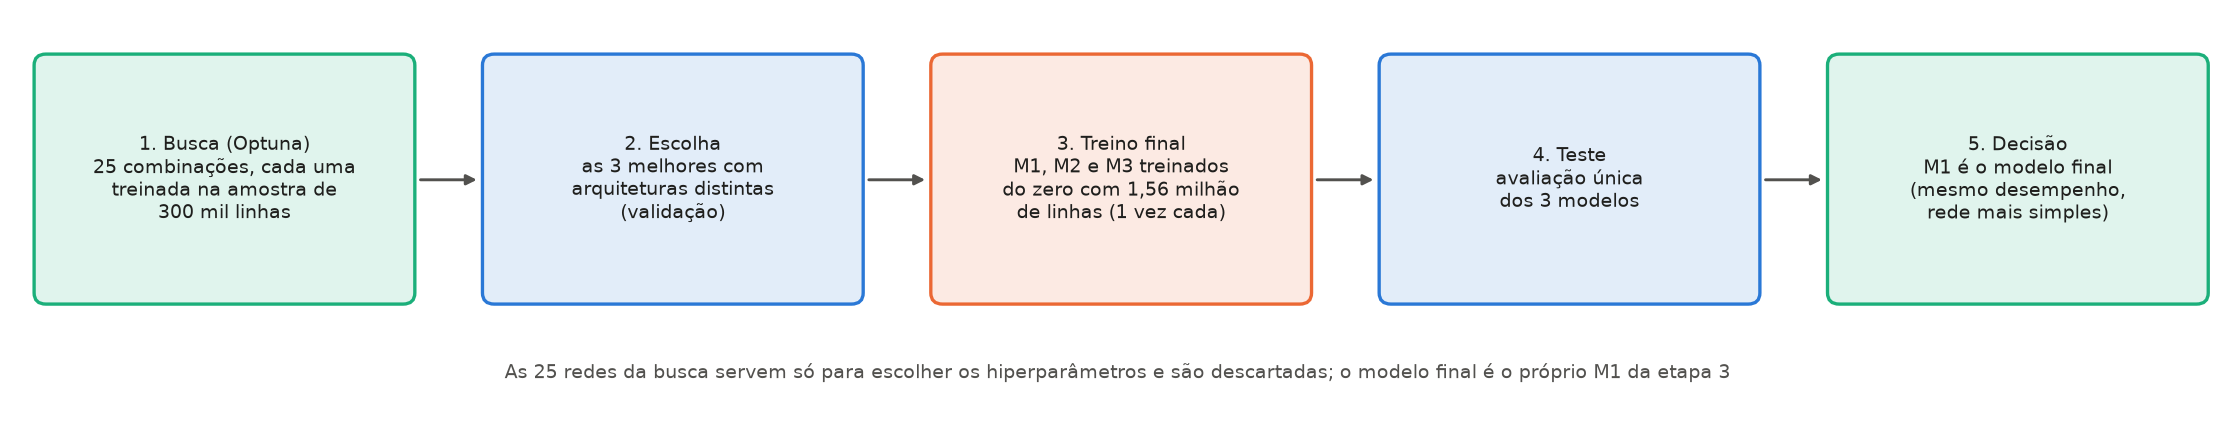
\includegraphics[width=0.7\textwidth]{figuras/19_fluxo_modelo_final}
  \caption{Da busca de hiperparâmetros ao modelo final}
  \label{fig:fluxo-final}
  \fontefig{Elaborado pelo autor}
\end{figure}

\chapter{Resultados de validação e seleção dos modelos promissores}
\label{cap:validacao}

\section{Resultados da hiperparametrização}
\label{sec:busca}

As 25 tentativas levaram 6,2 minutos (23 completas, 2 podadas). A Figura~\ref{fig:optuna} mostra a evolução da busca e a importância dos hiperparâmetros; a Tabela~\ref{tab:top5}, as cinco melhores tentativas. O espaço é pouco sensível perto do ótimo (as 17 melhores ficam entre 0,597 e 0,600), e o que mais prejudica é a regularização forte: as piores tentativas combinam L2 alto ($> 10^{-3}$) com taxa de aprendizado baixa, e L1 e L2 aparecem como os mais importantes na fANOVA por causa dessas falhas, não de sensibilidade perto do ótimo. O lote de 512 dominou a partir da tentativa 6 e o sobreajuste é pequeno em todas (\textit{gap} de Macro F1 abaixo de 0,016).

\begin{figure}[!htbp]
  \centering
  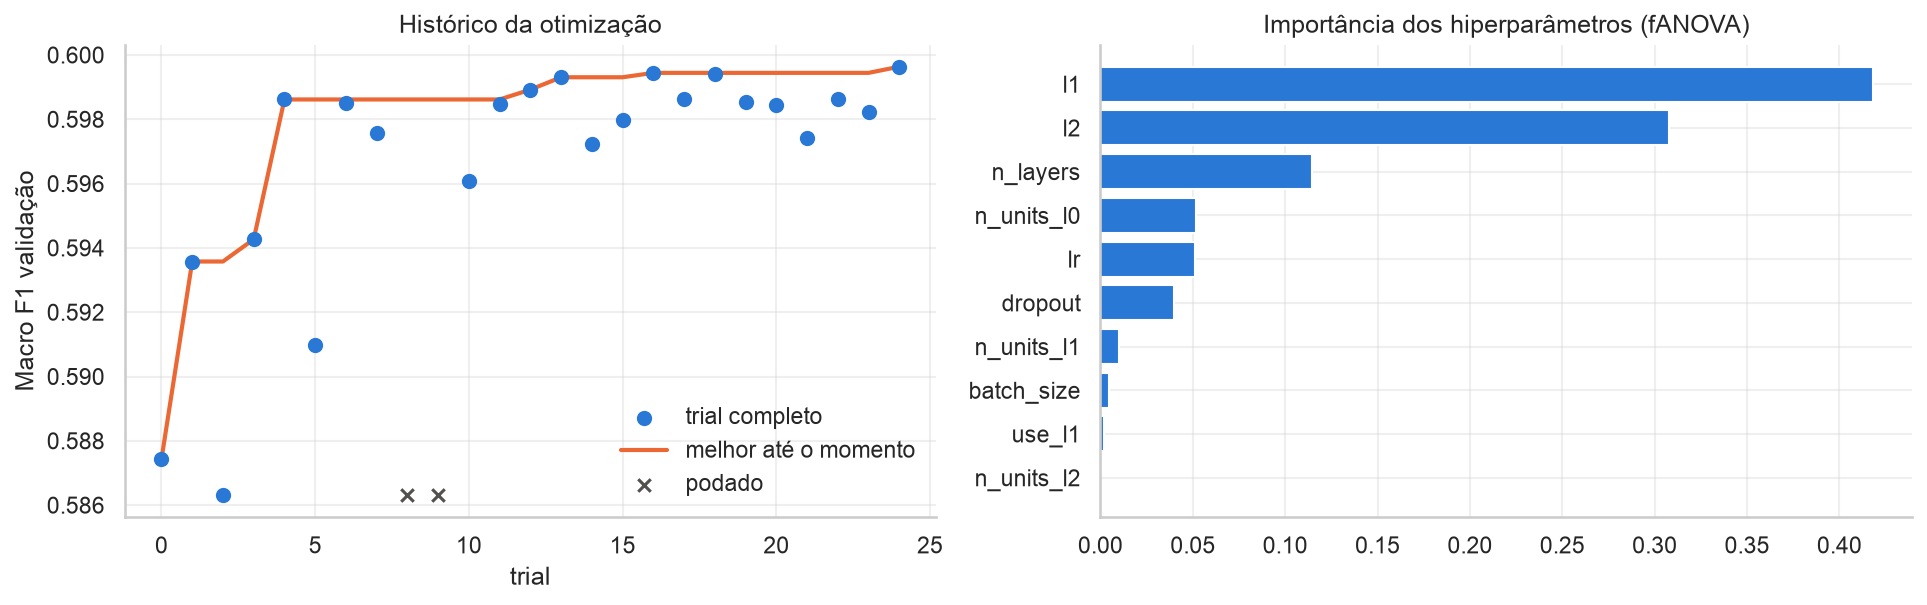
\includegraphics[width=0.7\textwidth]{figuras/10_optuna}
  \caption{Histórico da busca e importância dos hiperparâmetros (fANOVA)}
  \label{fig:optuna}
  \fontefig{Elaborado pelo autor}
\end{figure}

\begin{table}[!htbp]
\caption{Cinco melhores tentativas do Optuna (Macro F1 na validação)}
\label{tab:top5}
\begin{center}
\scriptsize
\setlength{\tabcolsep}{4pt}
\begin{tabular}{ccccccccc}
\hline
\textbf{Tentativa} & \makecell{\textbf{Macro F1}\\\textbf{val}} & \makecell{\textbf{Camadas}\\\textbf{ocultas}} & \textbf{Dropout} & \makecell{\textbf{Taxa de}\\\textbf{aprendizado}} & \textbf{L2} & \textbf{L1} & \textbf{Parâmetros} & \textbf{Gap F1} \\ \hline
24 & \textbf{0,5996} & 172 & 0,24 & $4{,}6 \cdot 10^{-4}$ & $1{,}1 \cdot 10^{-5}$ & --- & 34.059 & 0,008 \\
16 & 0,5994 & 215 $\rightarrow$ 25 & 0,32 & $7{,}2 \cdot 10^{-4}$ & $1{,}2 \cdot 10^{-5}$ & $1{,}3 \cdot 10^{-7}$ & 47.403 & 0,016 \\
18 & 0,5994 & 219 $\rightarrow$ 17 & 0,40 & $9{,}3 \cdot 10^{-4}$ & $8{,}0 \cdot 10^{-6}$ & $1{,}1 \cdot 10^{-7}$ & 46.499 & 0,008 \\
13 & 0,5993 & 228 $\rightarrow$ 19 & 0,17 & $4{,}8 \cdot 10^{-4}$ & $6{,}0 \cdot 10^{-5}$ & --- & 48.871 & 0,014 \\
12 & 0,5989 & 253 $\rightarrow$ 19 & 0,14 & $3{,}0 \cdot 10^{-4}$ & $5{,}0 \cdot 10^{-5}$ & --- & 54.221 & 0,012 \\ \hline
\end{tabular}
\end{center}
\fontetab{Elaborado pelo autor. Lote de 512 em todas. Gap F1 = Macro F1 de treino menos o de validação, na melhor época}
\end{table}

\section{Efeito da largura e da profundidade}
\label{sec:largura}

Para isolar o efeito da arquitetura, 9 redes foram treinadas na subamostra de 300 mil linhas variando só a profundidade (1, 2 ou 3 camadas) e a largura (32, 128 ou 256 neurônios), com os demais hiperparâmetros fixos (Figura~\ref{fig:largura-controlado}). A amplitude total é pequena (0,0044 de Macro F1) e, dentro dela, a largura pesa mais que a profundidade: com 32 neurônios as redes ficam entre 0,595 e 0,597 (subajuste leve), de 32 para 128 o ganho é de até 0,004, e de 128 para 256, de cerca de 0,001. Mais camadas não ajudam: com 128 ou 256 neurônios, 1 camada é igual ou melhor que 2 e 3, que atingem o melhor resultado na época 4 ou 5 e depois só aumentam o \textit{gap}. A rede 3 $\times$ 256 tem 182 mil parâmetros e não supera a 1 $\times$ 256, com 51 mil.

\begin{figure}[!htbp]
  \centering
  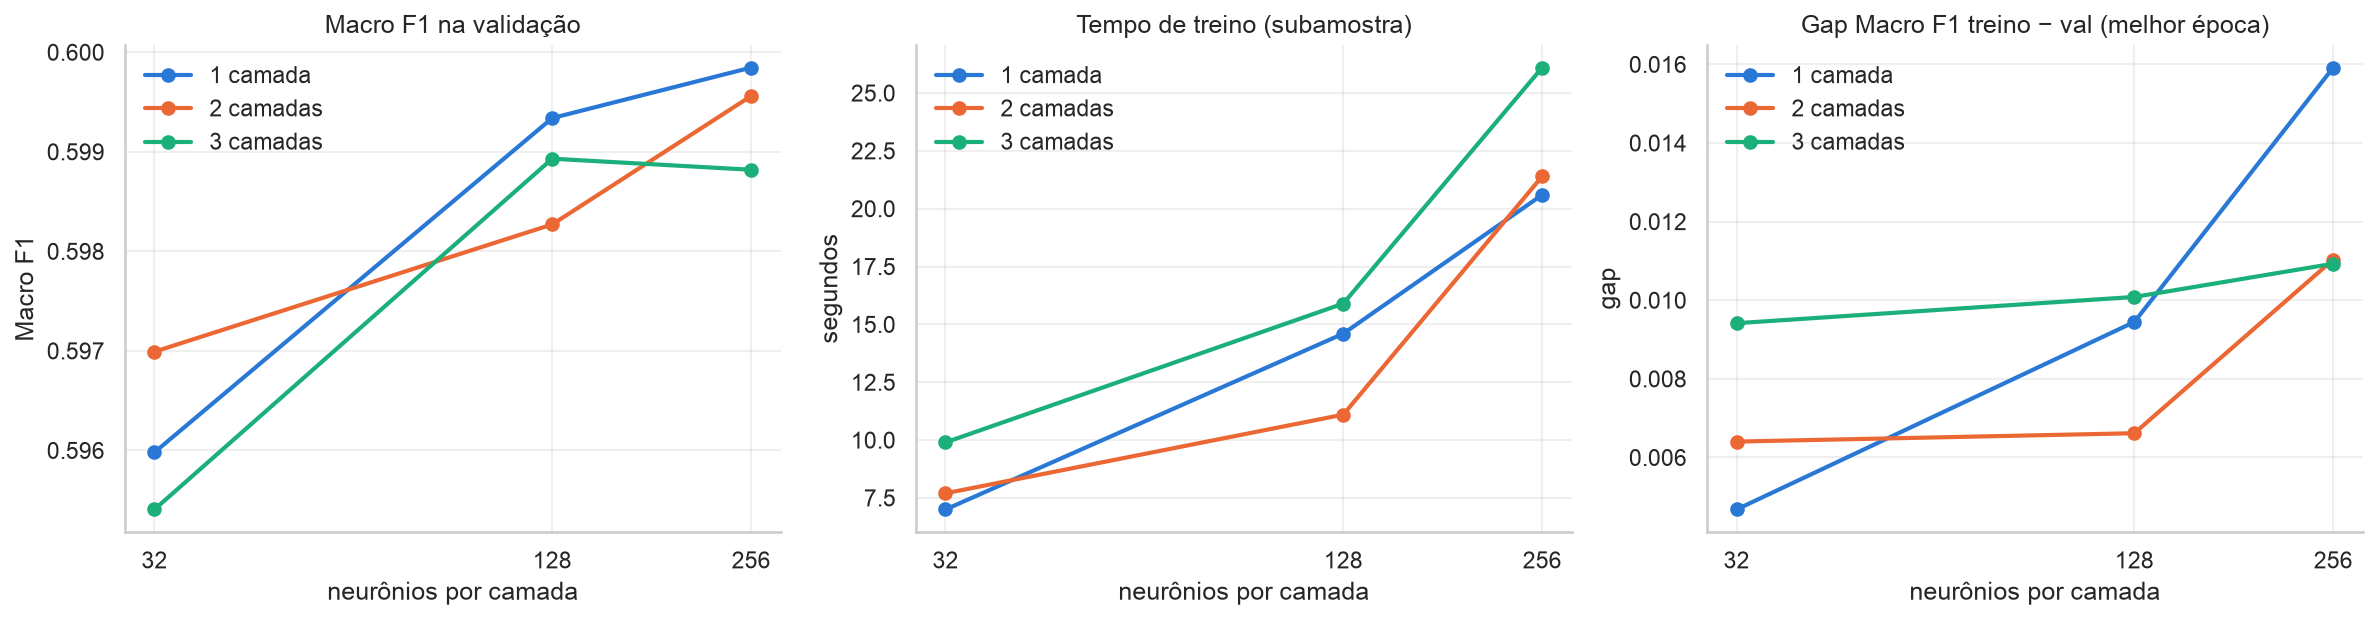
\includegraphics[width=0.85\textwidth]{figuras/10b_largura_profundidade_controlado}
  \caption{Experimento controlado de largura $\times$ profundidade (Macro F1 de validação, tempo e \textit{gap})}
  \label{fig:largura-controlado}
  \fontefig{Elaborado pelo autor}
\end{figure}

\section{Efeito da regularização}
\label{sec:regularizacao}

A arquitetura de M2 foi treinada na subamostra de 300 mil linhas por 25 épocas sem parada antecipada, com cada técnica isolada e com três referências (Tabela~\ref{tab:regularizacao} e Figura~\ref{fig:ablacao-reg}). Sem regularização a rede memoriza o treino (\textit{gap} de 0,060 e validação caindo após a 5\textsuperscript{a} época). O dropout é o que mais ajuda, e a combinação do Optuna é essencialmente esse dropout. L2 e L1 moderados reduzem o \textit{gap} sem melhorar a validação. O BatchNorm sozinho acelera o treino e antecipa o sobreajuste (melhor época 3, \textit{gap} de 0,094); não é regularização por si \cite{geron2019} e ficou fora dos finais. A regularização forte elimina o \textit{gap} à custa do desempenho: subajuste. Simulando a parada antecipada sobre essas curvas, a paciência 1 para cedo demais e perde até 0,008; com paciência 4 ou 5 as três configurações recuperam o melhor valor das 25 épocas, o que justifica os valores usados.

\begin{table}[!htbp]
\caption{Regularização técnica por técnica (25 épocas, sem parada antecipada)}
\label{tab:regularizacao}
\begin{center}
\scriptsize
\setlength{\tabcolsep}{3pt}
\begin{tabular}{P{3.3cm} c c c c P{4.6cm}}
\hline
\textbf{Configuração} & \makecell{\textbf{Macro F1}\\\textbf{treino}\\\textbf{(última)}} & \makecell{\textbf{Macro F1}\\\textbf{val}\\\textbf{(última)}} & \makecell{\textbf{Melhor}\\\textbf{Macro F1}\\\textbf{val (época)}} & \makecell{\textbf{Gap}\\\textbf{(última)}} & \textbf{Diagnóstico} \\ \hline
Sem regularização & 0,644 & 0,584 & 0,598 (5) & \textbf{0,060} & sobreajuste: o treino sobe sem parar e a validação cai depois da 5\textsuperscript{a} época \\ \hline
Só dropout (0,32) & 0,630 & 0,595 & 0,599 (12) & 0,034 & técnica isolada mais eficaz \\ \hline
Só L2 ($10^{-4}$) & 0,627 & 0,589 & 0,598 (6) & 0,039 & reduz o \textit{gap}, mas a validação ainda cai \\ \hline
Só L1 ($10^{-5}$) & 0,622 & 0,591 & 0,598 (8) & 0,031 & efeito parecido com o do L2 \\ \hline
Só BatchNorm & 0,667 & 0,573 & 0,596 (3) & \textbf{0,094} & antecipa o sobreajuste \\ \hline
Combinação do Optuna (dropout 0,32, L2 $1{,}2 \cdot 10^{-5}$, L1 $1{,}3 \cdot 10^{-7}$) & 0,626 & 0,597 & \textbf{0,600} (16) & 0,030 & equilíbrio: menor \textit{gap} sem subajuste e melhor validação \\ \hline
Regularização forte (dropout 0,5, L2 $10^{-2}$) & 0,565 & 0,564 & 0,578 (15) & 0,001 & subajuste: treino e validação colados e baixos \\ \hline
\end{tabular}
\end{center}
\fontetab{Elaborado pelo autor}
\end{table}

\begin{figure}[!htbp]
  \centering
  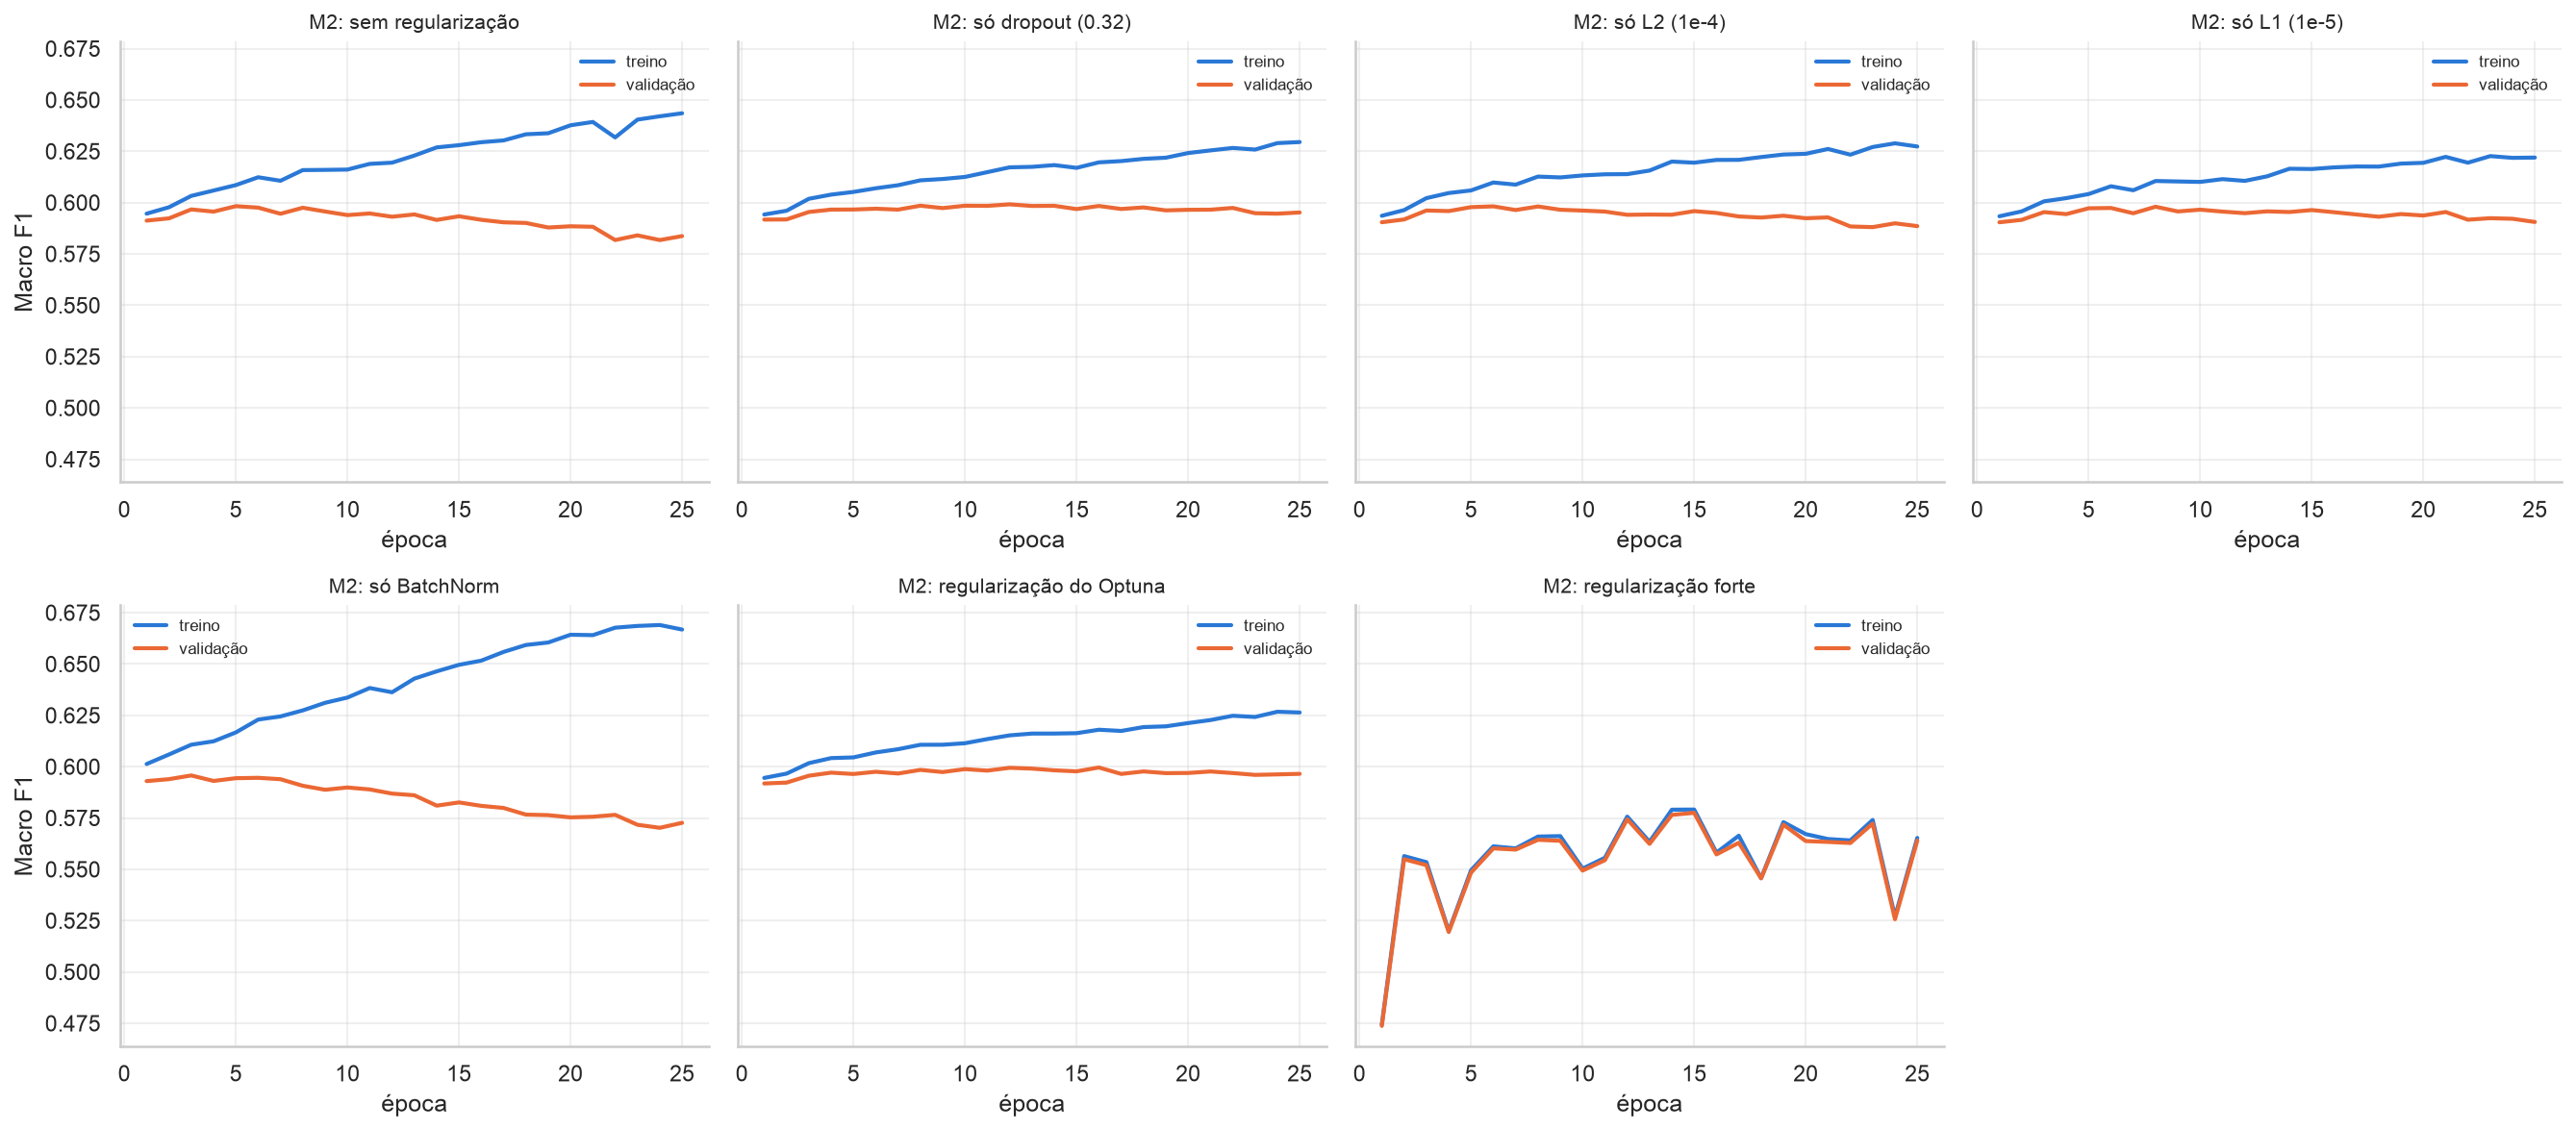
\includegraphics[width=0.7\textwidth]{figuras/13_ablacao_regularizacao}
  \caption{Macro F1 de treino e validação por época, por técnica de regularização}
  \label{fig:ablacao-reg}
  \fontefig{Elaborado pelo autor}
\end{figure}

\section{Seleção dos modelos finalistas}
\label{sec:finalistas}

As três melhores tentativas com arquiteturas distintas (24, 16 e 18 na Tabela~\ref{tab:top5}) definem os finalistas M1, M2 e M3 (Quadro~\ref{qua:finais}). A busca convergiu para redes rasas e largas: uma camada de 172 neurônios ou duas camadas em formato pirâmide (cerca de 215 e 20 neurônios), sempre com dropout entre 0,24 e 0,40, L2 em torno de $10^{-5}$, L1 desligado ou quase nulo e lote 512. Três variações são comparadas para verificar se a segunda camada traz algum ganho no treino com a base completa.

\begin{quadro}[!htbp]
\caption{Arquiteturas finalistas resultantes da hiperparametrização}
\label{qua:finais}
\begin{center}
\scriptsize
\setlength{\tabcolsep}{4pt}
\begin{tabular}{|c|c|c|c|c|c|c|c|}
\hline
\textbf{Modelo} & \textbf{Tentativa} & \textbf{Arquitetura} & \textbf{Parâmetros} & \textbf{Dropout} & \makecell{\textbf{Taxa de}\\\textbf{aprendizado}} & \textbf{L2} & \textbf{L1} \\ \hline
M1 & 24 & 194 $\rightarrow$ 172 $\rightarrow$ 3 & 34.059 & 0,24 & $4{,}6 \cdot 10^{-4}$ & $1{,}1 \cdot 10^{-5}$ & --- \\ \hline
M2 & 16 & 194 $\rightarrow$ 215 $\rightarrow$ 25 $\rightarrow$ 3 & 47.403 & 0,32 & $7{,}2 \cdot 10^{-4}$ & $1{,}2 \cdot 10^{-5}$ & $1{,}3 \cdot 10^{-7}$ \\ \hline
M3 & 18 & 194 $\rightarrow$ 219 $\rightarrow$ 17 $\rightarrow$ 3 & 46.499 & 0,40 & $9{,}3 \cdot 10^{-4}$ & $8{,}0 \cdot 10^{-6}$ & $1{,}1 \cdot 10^{-7}$ \\ \hline
\end{tabular}
\end{center}
\fontequa{Elaborado pelo autor. Arquitetura: entrada $\rightarrow$ camadas ocultas $\rightarrow$ saída; ReLU nas ocultas, softmax na saída, Adam e lote 512 em todos}
\end{quadro}

\chapter{Avaliação no conjunto de teste e custo versus efetividade}
\label{cap:teste}

\section{Desempenho e custo dos modelos finais}
\label{sec:finais}

Treinados com toda a base de treino e avaliados no teste, M1 e M2 empatam em Macro F1 (0,6065) e M3 fica 0,002 abaixo (Tabela~\ref{tab:finais} e Figura~\ref{fig:custo}). M1 também teve o melhor Macro F1 de validação (0,6046); com uma única semente por modelo, diferenças dessa ordem não são significativas, e o fator decisivo é o custo: M1 foi escolhido por ter o mesmo desempenho com a menor rede (28\% menos parâmetros que M2, uma única camada oculta) e um quinto do tempo de treino de M2. A inferência é desprezível nos três: cerca de 0,1 s para 334 mil acidentes em CPU.

\begin{table}[!htbp]
\caption{Desempenho e custo dos modelos finais no teste}
\label{tab:finais}
\begin{center}
\scriptsize
\setlength{\tabcolsep}{4pt}
\begin{tabular}{cccccccccc}
\hline
\textbf{Modelo} & \textbf{Parâmetros} & \makecell{\textbf{Épocas}\\\textbf{(melhor)}} & \makecell{\textbf{Treino}\\\textbf{(s)}} & \makecell{\textbf{Inferência}\\\textbf{(ms)}} & \textbf{Acurácia} & \makecell{\textbf{Precisão}\\\textbf{macro}} & \makecell{\textbf{\textit{Recall}}\\\textbf{macro}} & \textbf{Macro F1} & \makecell{\textbf{Macro F1}\\\textbf{val}} \\ \hline
\textbf{M1} & 34.059 & 22 (17) & 119 & 126 & \textbf{0,7029} & 0,6020 & 0,6140 & \textbf{0,6065} & 0,6046 \\
M2 & 47.403 & 13 (8) & 580 & 98 & \textbf{0,7029} & 0,6034 & 0,6142 & \textbf{0,6065} & 0,6041 \\
M3 & 46.499 & 8 (3) & 261 & 98 & 0,7023 & 0,6051 & 0,6077 & 0,6041 & 0,6017 \\ \hline
\end{tabular}
\end{center}
\fontetab{Elaborado pelo autor. Inferência sobre os 333.798 exemplos do teste, em CPU}
\end{table}

\begin{figure}[!htbp]
  \centering
  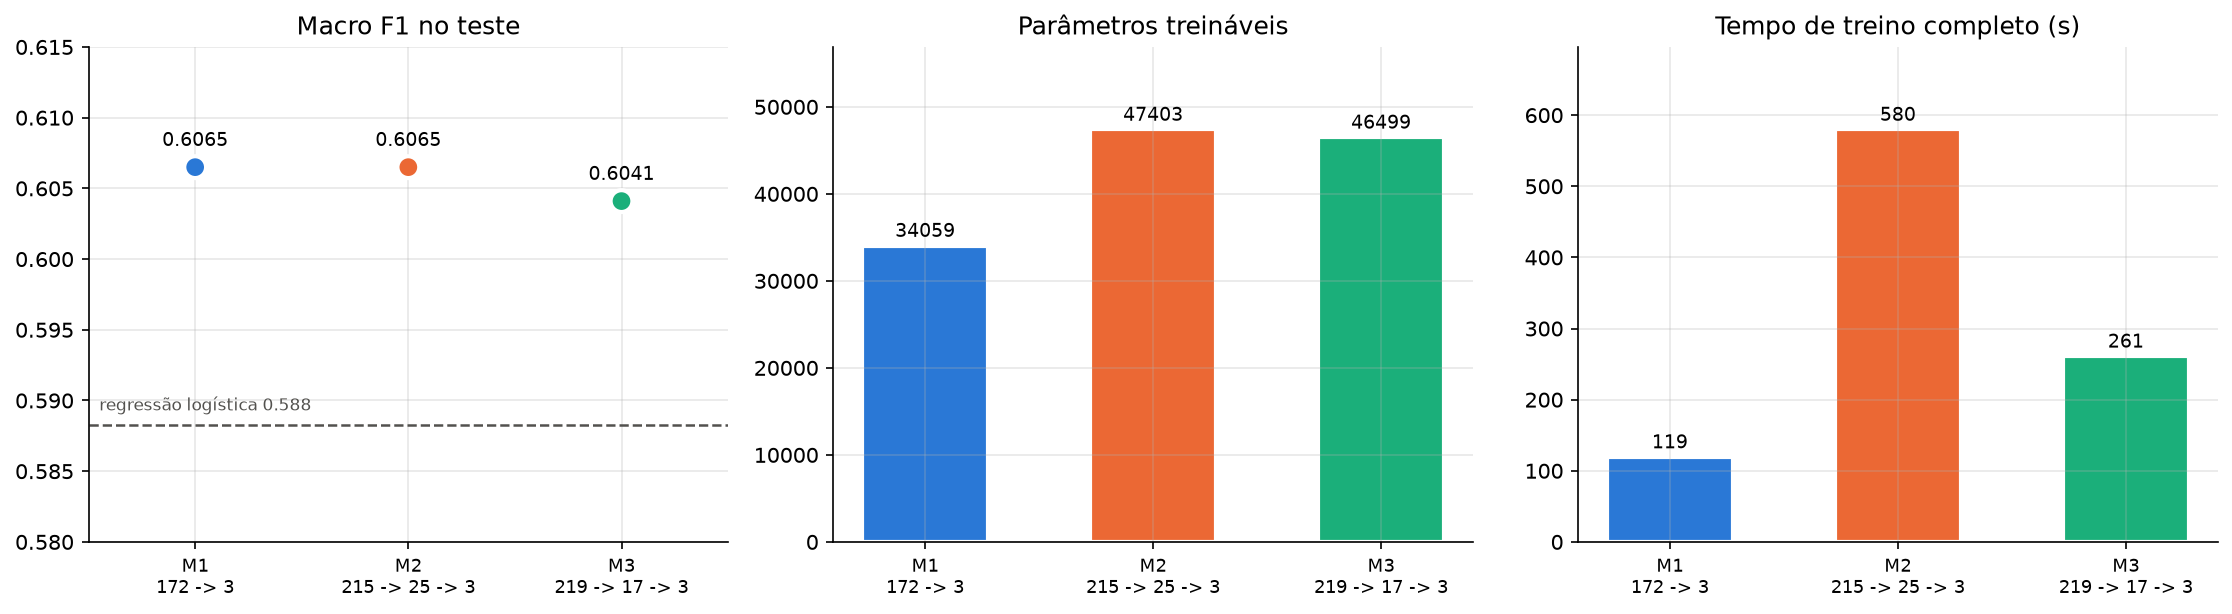
\includegraphics[width=0.65\textwidth]{figuras/18_custo_efetividade}
  \caption{Macro F1 no teste, parâmetros e tempo de treino dos modelos finais}
  \label{fig:custo}
  \fontefig{Elaborado pelo autor}
\end{figure}

A Figura~\ref{fig:confusao} mostra as matrizes de confusão do M1. \texttt{Sem Vítimas} é a classe mais fácil (\textit{recall} de 78\%); o erro mais comum é entre \texttt{Sem Vítimas} e \texttt{Com Vítimas Feridas}, que têm relatos parecidos. Dos acidentes fatais, 40\% são reconhecidos (precisão 0,36, F1 0,38), 46\% vão para \texttt{Com Vítimas Feridas} e 14\% para \texttt{Sem Vítimas}: 86\% dos fatais são sinalizados como \aspas{com vítima}, o que já aciona o socorro, e os 14\% restantes são o erro mais grave do modelo.

\begin{figure}[!htbp]
  \centering
  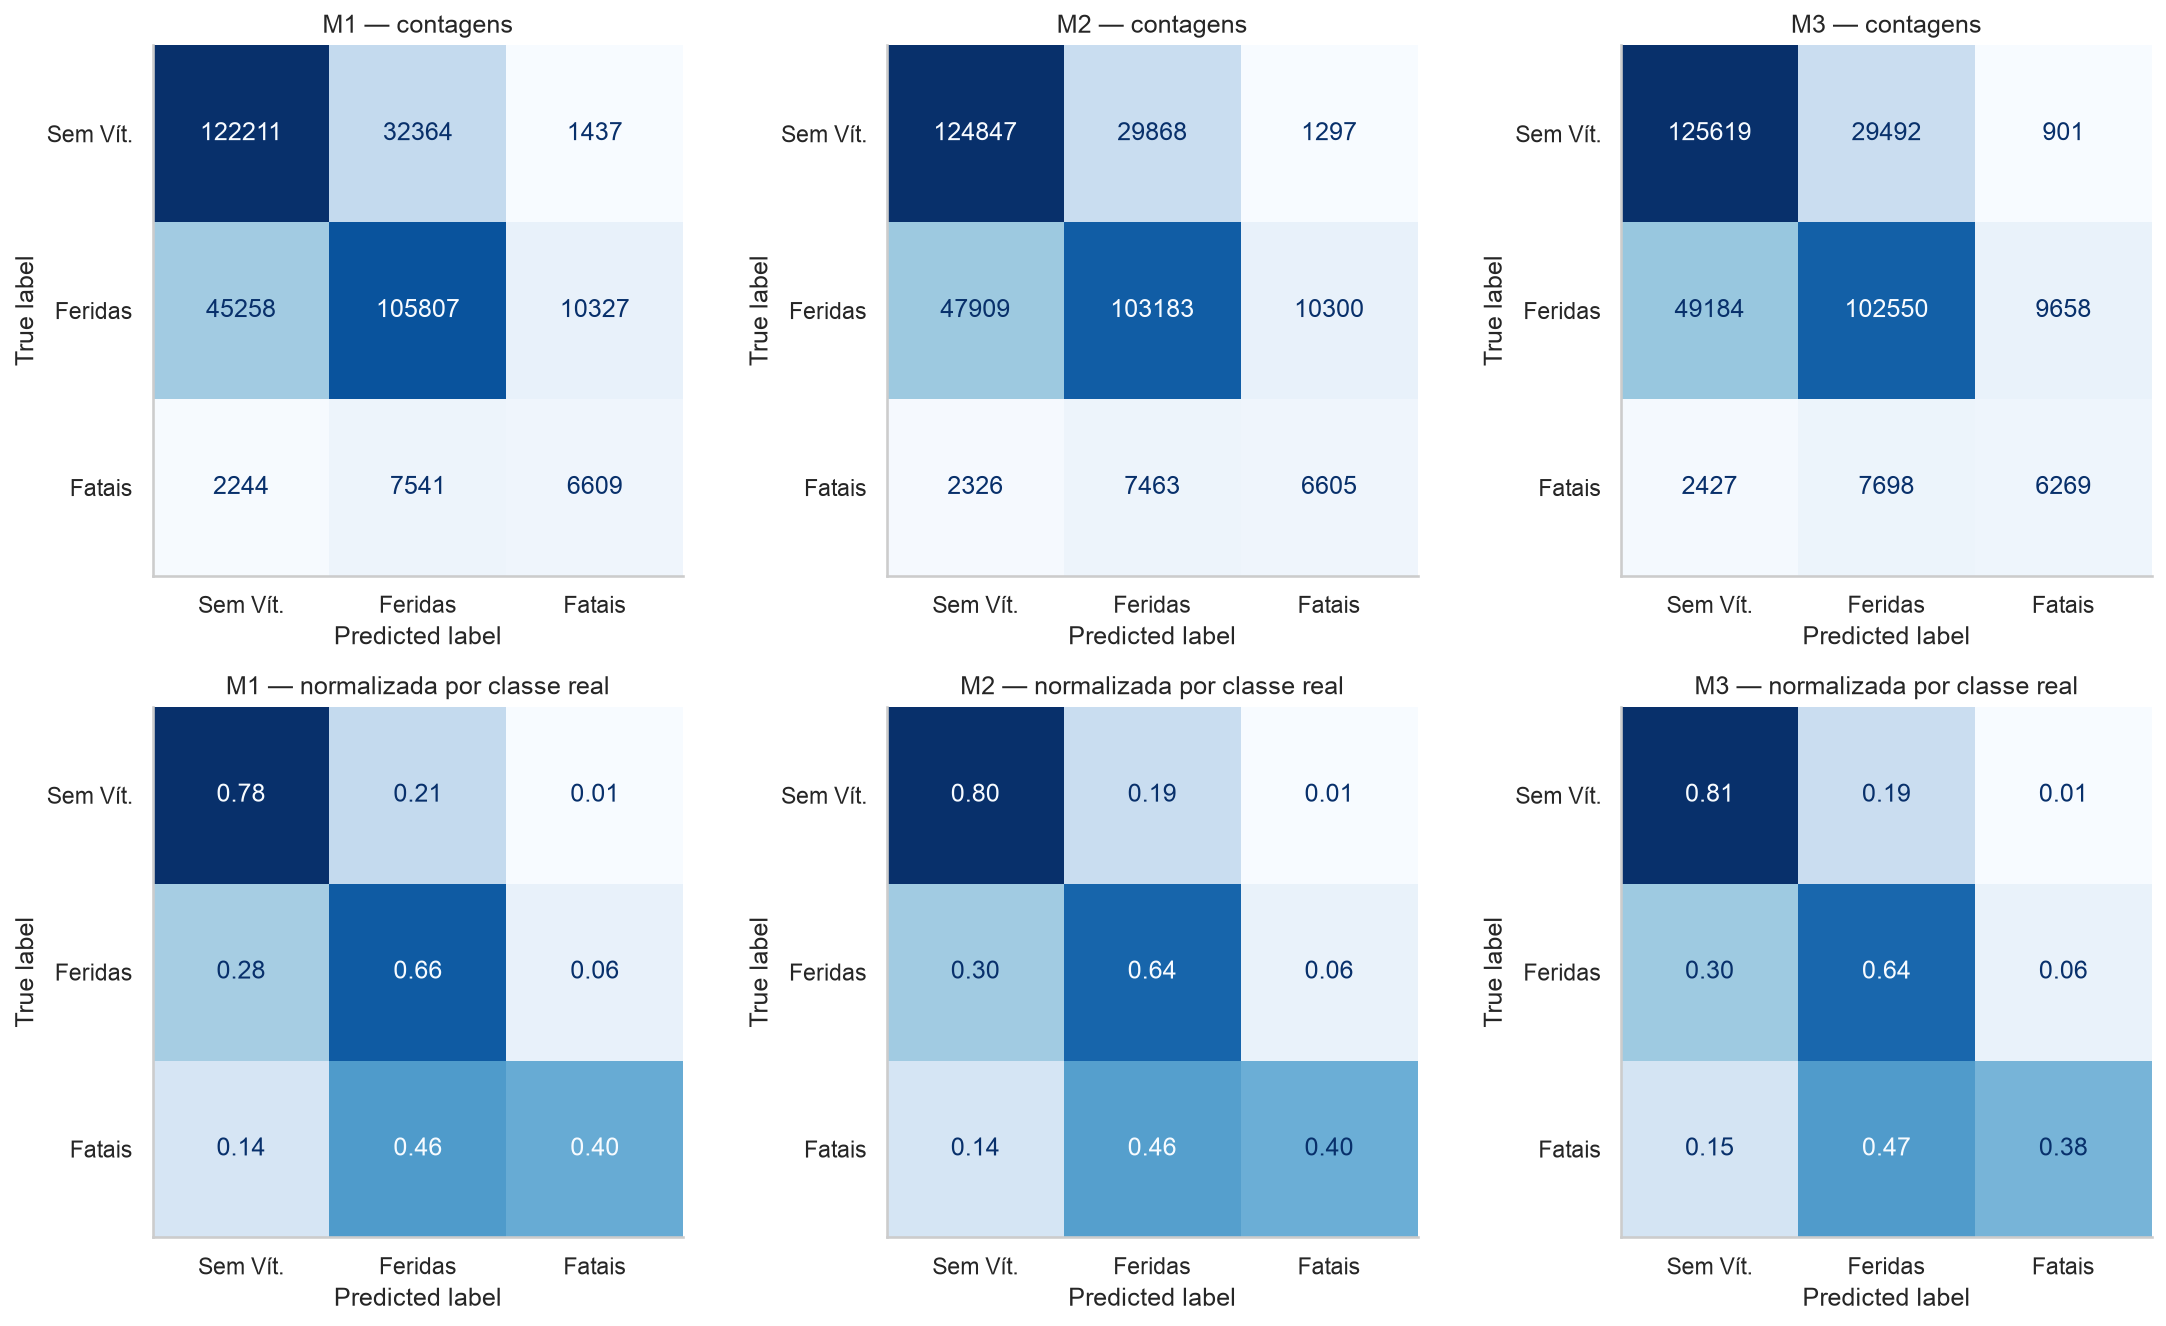
\includegraphics[width=0.5\textwidth]{figuras/11_matrizes_confusao}\hfill
  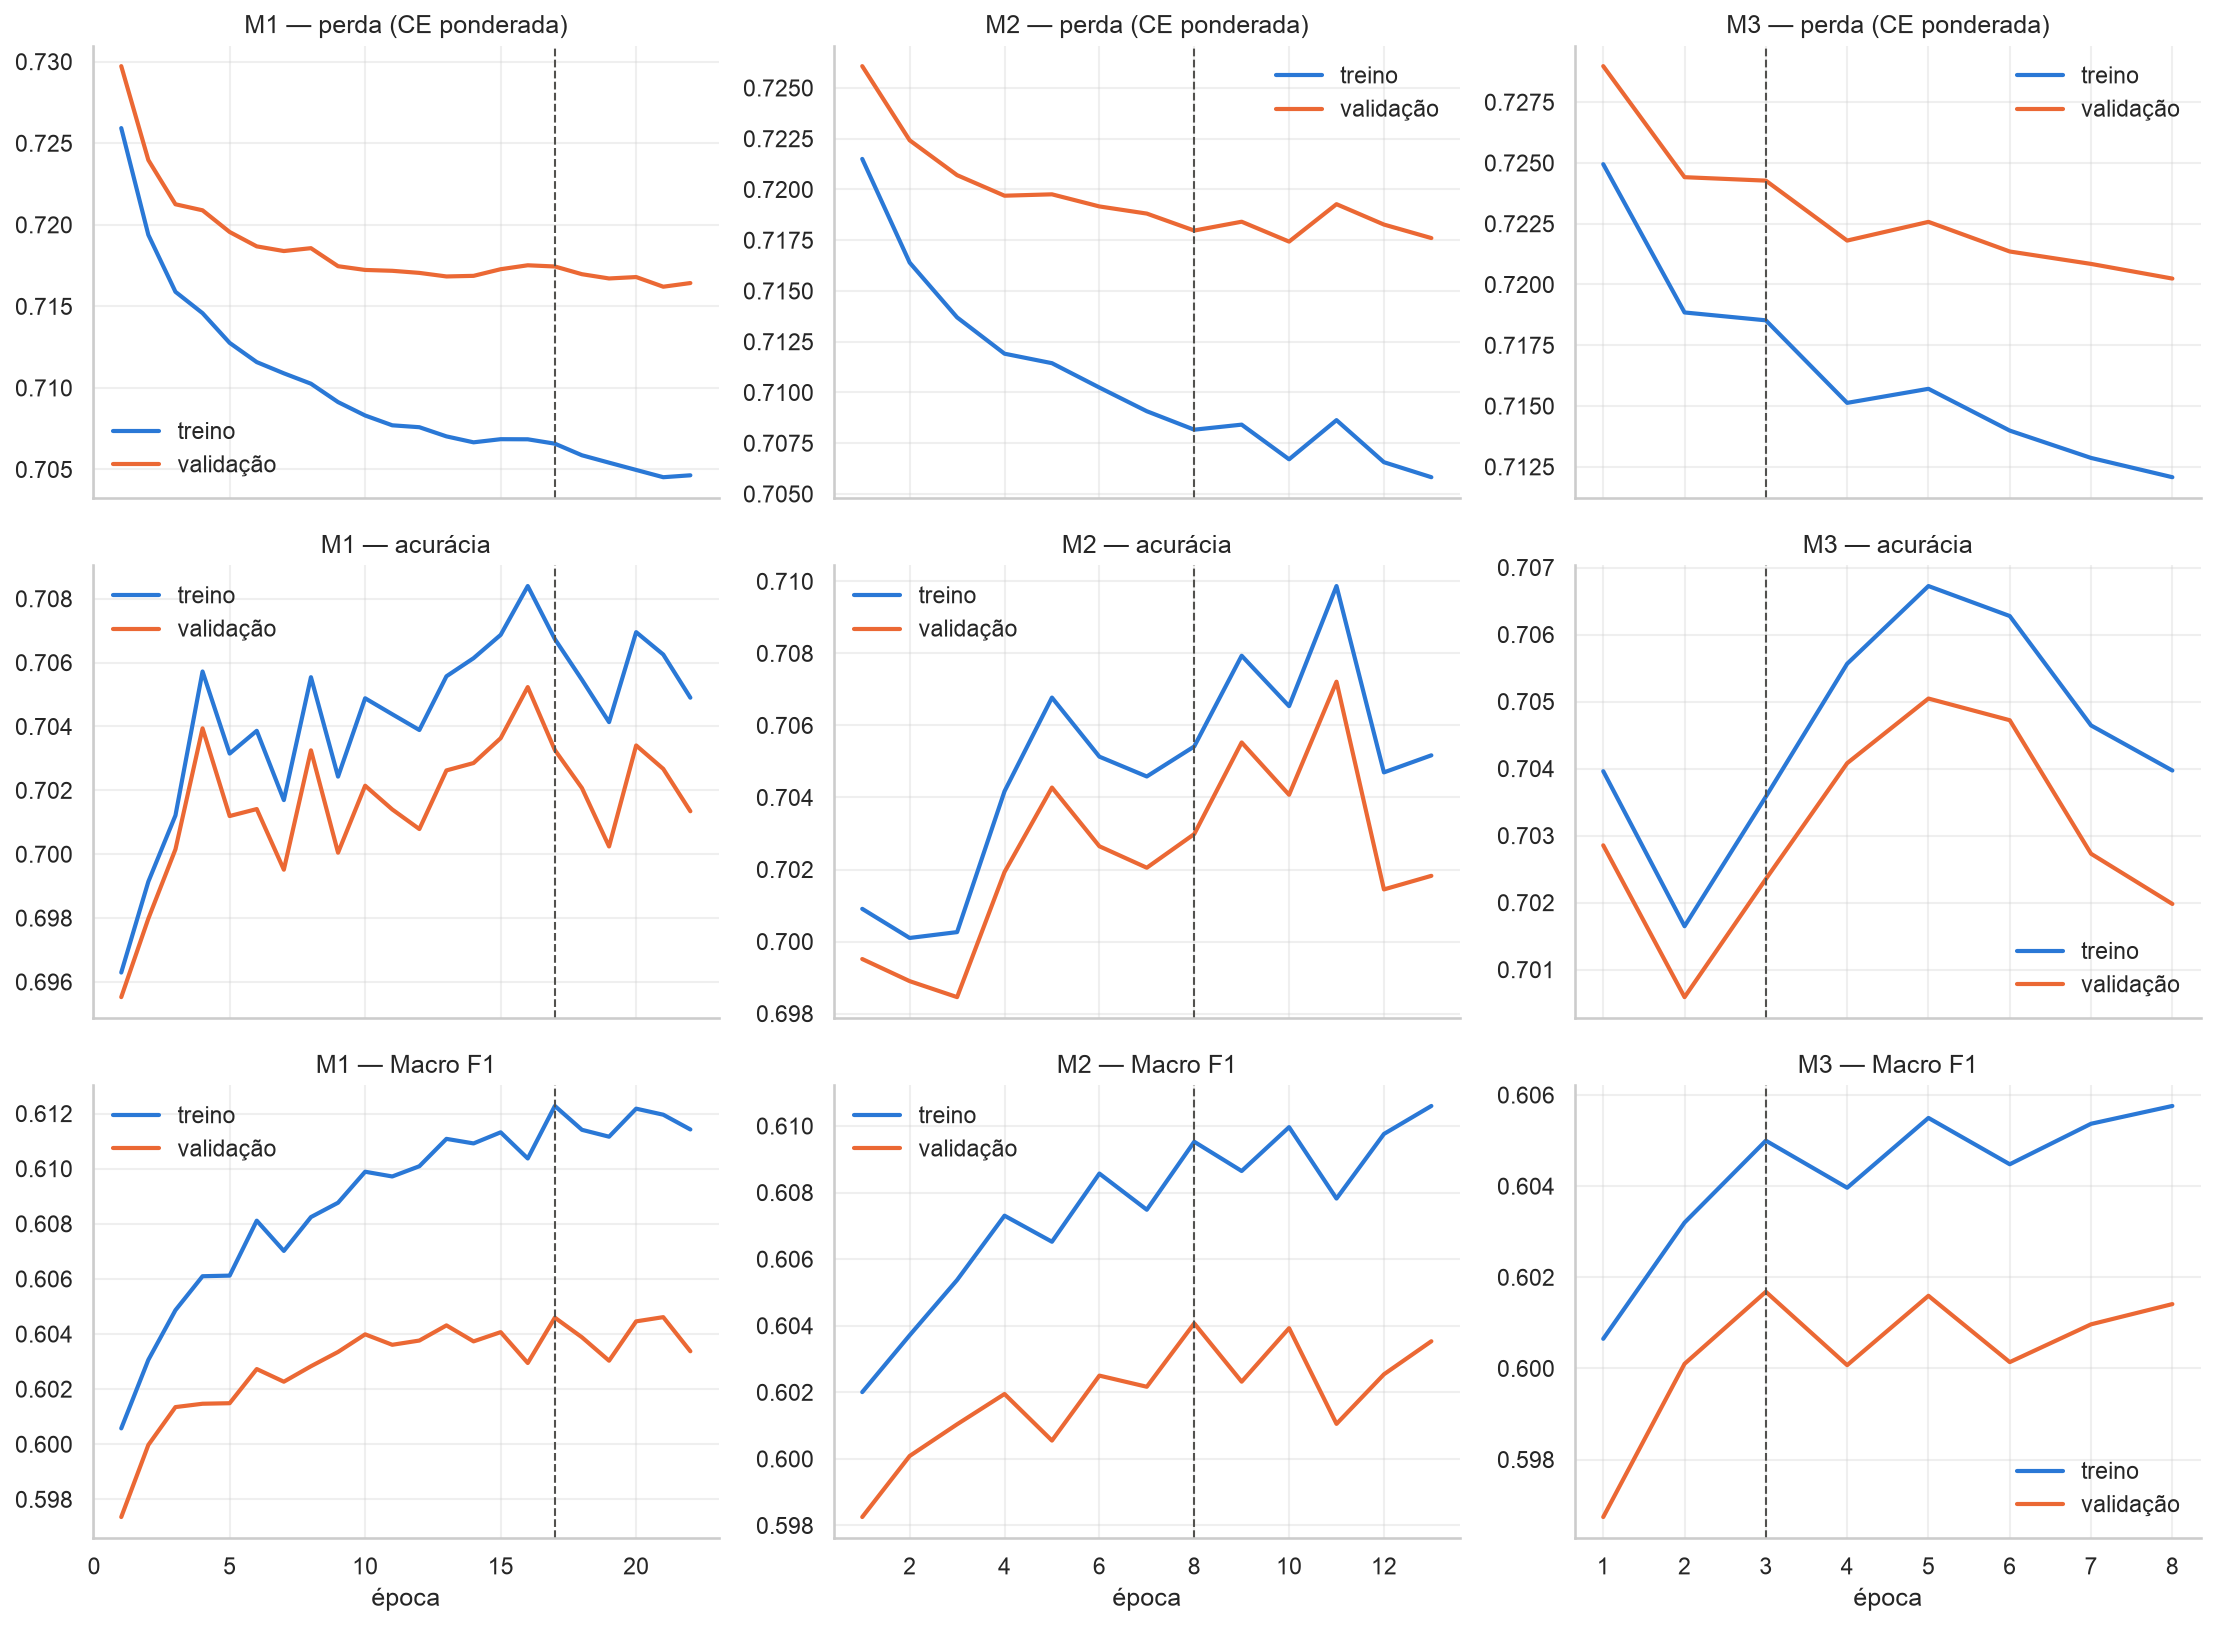
\includegraphics[width=0.42\textwidth]{figuras/12_curvas_treino_validacao}
  \caption{À esquerda, matrizes de confusão do M1 no teste, em contagens e normalizadas pela classe real; à direita, perda, acurácia e Macro F1 por época dos finalistas, com a linha tracejada na melhor época}
  \label{fig:confusao}
  \fontefig{Elaborado pelo autor}
\end{figure}

\section{Curvas de treino e validação}
\label{sec:curvas}

Nas curvas dos três finalistas (Figura~\ref{fig:confusao}, à direita), a perda de treino e a de validação caem juntas, e o Macro F1 de validação para de melhorar e oscila (melhor época 17 no M1, 8 no M2 e 3 no M3), o que dispara a parada antecipada. O sobreajuste é leve: o \textit{gap} de Macro F1 na melhor época fica entre 0,003 e 0,008, menor no M3, que tem o maior dropout. Não há subajuste: o teto de cerca de 70\% de acurácia vem das entradas (Seção~\ref{sec:baselines}), não da capacidade da rede. Já o \textit{recall} de 40\% nos fatais é o ponto de operação dos pesos de classe, não um teto: um peso maior elevaria o \textit{recall} à custa da precisão.


\section{Comparação com \textit{baselines} e ablação por grupo de entradas}
\label{sec:baselines}

A MLP supera a regressão logística (com \texttt{C} escolhido na validação) em 1,8 p.p. de acurácia e de Macro F1 (Tabela~\ref{tab:baselines}): um ganho real, mas pequeno, vindo da combinação não linear das mesmas entradas. A ablação (Figura~\ref{fig:ablacao-grupos}) mostra de onde vem o desempenho: só com o contexto da via a MLP empata com a tabela de frequências (52,9\%) e nunca prevê fatal; local e horário acrescentam 2,9 p.p.; o relato do solicitante acrescenta 14,6 p.p. e é o que faz a classe fatal ser reconhecida (\textit{recall} de 0 para 0,40). As entradas pesam muito mais que a arquitetura; o efeito isolado de \texttt{macro\_causa}, a única do grupo que não vem do solicitante, não foi medido.

\begin{table}[!htbp]
\caption{Comparação com \textit{baselines} no teste}
\label{tab:baselines}
\begin{center}
\footnotesize
\begin{tabularx}{\textwidth}{Y c c}
\hline
\textbf{Modelo} & \textbf{Acurácia} & \textbf{Macro F1} \\ \hline
Classe majoritária & 0,484 & 0,217 \\
Sorteio proporcional às classes & 0,455 & 0,334 \\
Tabela de frequências só com o contexto da via (414 combinações) & 0,529 & 0,361 \\
Regressão logística (12 entradas, $C = 1$) & 0,685 & 0,588 \\
\textbf{MLP M1} & \textbf{0,703} & \textbf{0,607} \\ \hline
\end{tabularx}
\end{center}
\fontetab{Elaborado pelo autor}
\end{table}

\begin{figure}[!htbp]
  \centering
  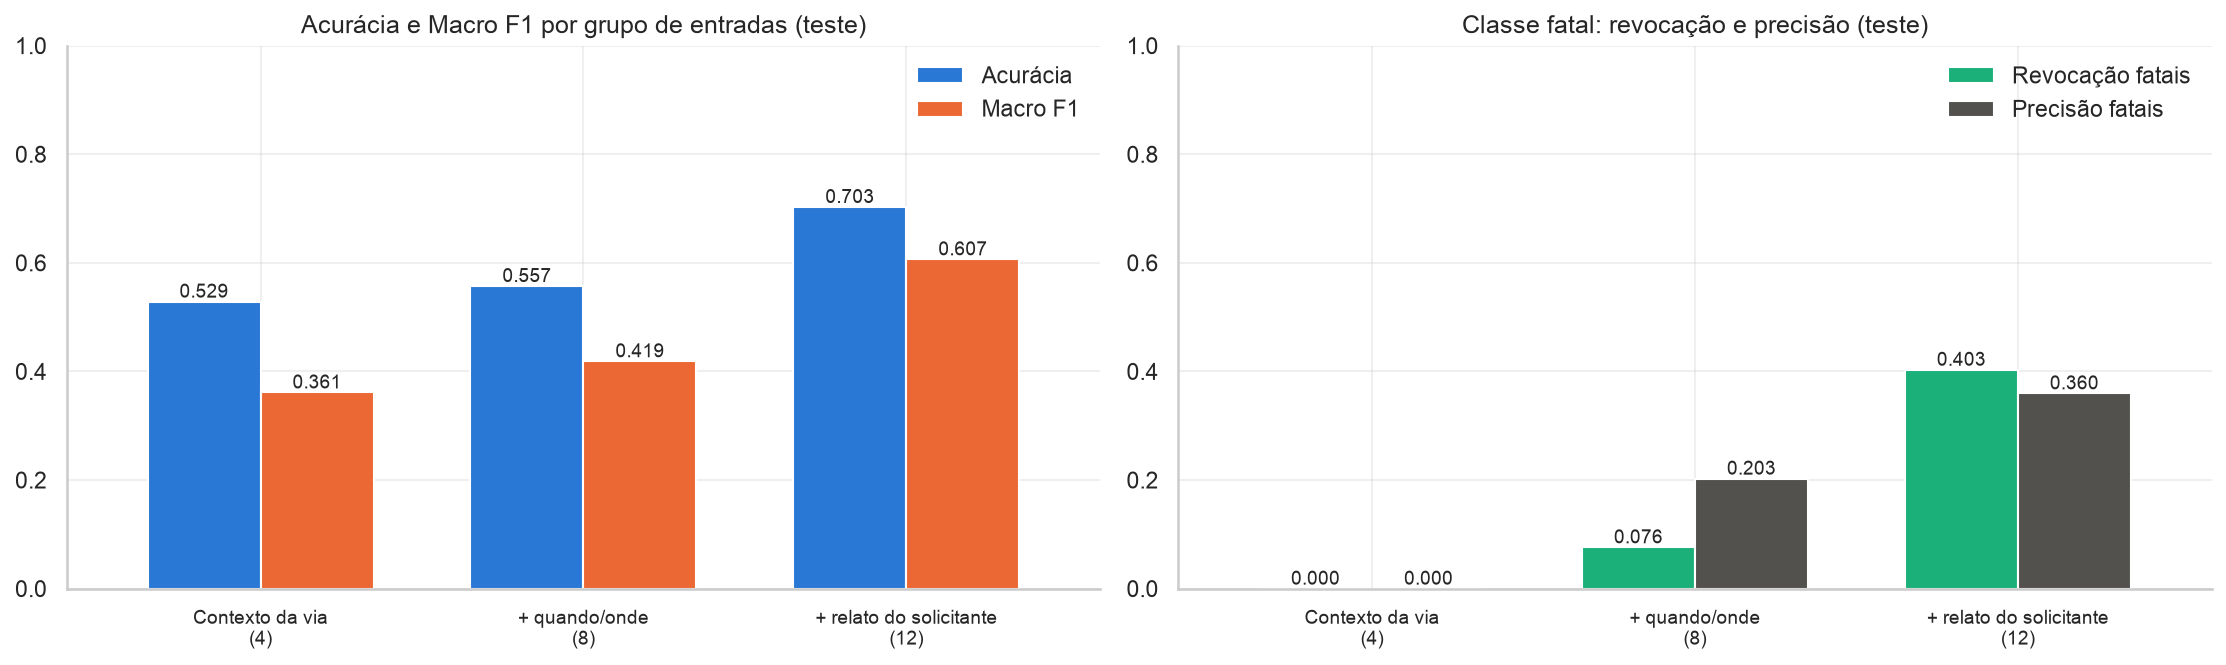
\includegraphics[width=0.7\textwidth]{figuras/14_ablacao_grupos_entradas}
  \caption{Arquitetura de M1 treinada com grupos crescentes de entradas (teste)}
  \label{fig:ablacao-grupos}
  \fontefig{Elaborado pelo autor}
\end{figure}

\chapter{Limitações e conclusões}
\label{cap:conclusao}

\section{Limitações}
\label{sec:limitacoes}

\begin{itemize}
  \item \textbf{Dois regimes de registro.} A categoria \texttt{nao informada} de \texttt{macro\_causa} ainda marca o período anterior a 2017, e a divisão aleatória mistura os dois regimes no teste; um teste cronológico mediria melhor o uso futuro.
  \item \textbf{Disponibilidade das entradas.} A causa provável é avaliação da equipe, não do solicitante; não se sabe quanto do ganho do grupo relato depende dela.
  \item \textbf{Classe fatal.} Com 40\% de \textit{recall}, o modelo deixa passar 6 em cada 10 fatais: serve para priorizar, nunca para negar socorro. Esse valor é o ponto de operação dos pesos de classe, não um limite do modelo.
  \item \textbf{Qualidade do relato.} O modelo supõe que o solicitante informa corretamente tipo de acidente, pessoas e veículos, justamente as entradas mais importantes.
  \item \textbf{Uma única divisão e uma única semente.} Sem validação cruzada nem repetição do treino não há intervalo de confiança; diferenças de 0,002 entre os finalistas não são significativas.
  \item \textbf{Escolhas não otimizadas.} O expoente dos pesos de classe e a paciência ficaram fora da busca; a busca e os experimentos de arquitetura e regularização usaram uma subamostra de 300 mil linhas.
\end{itemize}

\section{Conclusões}
\label{sec:conclusao}

Uma MLP com uma camada oculta de 172 neurônios (34 mil parâmetros) classifica a gravidade de acidentes em rodovias federais com 70,3\% de acurácia e Macro F1 de 0,607 no teste, contra 48\% da classe majoritária e 68,5\% da regressão logística.

A hiperparametrização mostrou que o desempenho é pouco sensível à arquitetura perto do ótimo e que a regularização forte é o que mais prejudica. Dentro do intervalo explorado, a largura importa até cerca de 128 neurônios e mais camadas não ajudam neste problema tabular. O dropout foi a regularização mais eficaz, o BatchNorm sozinho só antecipou o sobreajuste, e a parada antecipada com paciência de 4 ou 5 épocas protegeu o resultado em todos os casos.

O principal limite está nas entradas, não na rede: o relato do solicitante responde por cerca de 15 pontos percentuais de acurácia. Como trabalhos futuros ficam medir o efeito isolado da causa provável, repetir o treino com várias sementes, tratar as classes como ordinais, definir o peso ou o limiar da classe fatal pelo custo de cada erro e avaliar o modelo num teste temporal.


% Referências (arquivo bib/bibliografia.bib, estilo ABNT autor-data)
\FloatBarrier
\clearpage
\bibliografia

\end{document}
